\begin{section}{Archimedes' Principle}
    Archimedes' principle can be found in several general physics textbooks, like
    \cite{RESNICK} and it states: 
    
    \textit{``A body wholly or partially immersed in a fluid will be buoyed up by a 
            force equal to the weight of the fluid that the body displaces"}
    
    make a discussion about the principle and how it matches the phenomenology 
    explained in the previous section linking it with newton's second law...for this
    purposes considere next pic,
    
    \begin{center}
        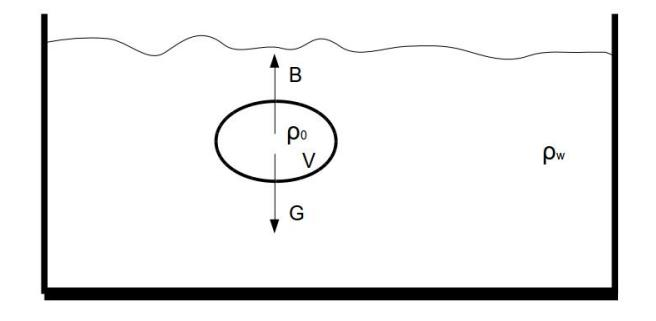
\includegraphics[scale=0.4]{./pics/buoyancy.jpg}
    \end{center}
       
\end{section}
